\documentclass[conference]{IEEEtran}
\usepackage{cite}
\usepackage{amsmath,amssymb,amsfonts}
% \usepackage{algorithmic}
\usepackage{graphicx}
\usepackage{textcomp}
\usepackage{xcolor}
\usepackage{fancyhdr}
\usepackage{algorithm}
\usepackage{algpseudocode}
\usepackage[hyphens]{url}

\def\BibTeX{{\rm B\kern-.05em{\sc i\kern-.025em b}\kern-.08em
    T\kern-.1667em\lower.7ex\hbox{E}\kern-.125emX}}

% Ensure letter paper
\pdfpagewidth=8.5in
\pdfpageheight=11in


\fancypagestyle{firstpage}{
  \fancyhf{}
\renewcommand{\headrulewidth}{0pt}
  \fancyhead[C]{CSE240A} 
  \fancyfoot[C]{\thepage}
}  


\pagenumbering{arabic}

%%%%%%%%%%%---SETME-----%%%%%%%%%%%%%
\title{Branch Predictor Project Report} 
\author{Pisit Wajanasara\\
PID: A59009987\\
University of California, San Diego}
%%%%%%%%%%%%%%%%%%%%%%%%%%%%%%%%%%%%

\begin{document}
\maketitle
\thispagestyle{firstpage}
\pagestyle{plain}



%%%%%% -- PAPER CONTENT STARTS-- %%%%%%%%

\begin{abstract}

This document is intended to serve as a sample for submissions to the
47th IEEE/ACM International Symposium on Computer Architecture (ISCA),
May 30 -- June 3, 2020 in Valencia, Spain. This document provides
guidelines that authors should follow when submitting papers to the
conference.  This format is derived from the IEEE conference template IEEEtran.cls
file with the objective of keeping the submission similar to the final
version, i.e., the IEEEtran.cls template will also be used for
  the camera-ready version.

\end{abstract}

\section{Introduction}

This document provides instructions for submitting papers to ISCA
2020.  In an effort to respect the efforts of reviewers and in the
interest of fairness to all prospective authors, we request that all
submissions to ISCA 2020 follow the formatting and submission rules
detailed below. Submissions that violate these instructions may not be
reviewed, at the discretion of the program chair, in order to
maintain a review process that is fair to all potential authors. This
document is itself formatted using the ISCA 2020 submission format. The
content of this document mirrors that of the submission instructions
that appear on the conference website. All questions regarding paper
formatting and submission should be directed to the program chair.

\section{Background}

\section{Design Ideas}

Our design is based mostly on tournament branch predictor used in Alpha 21264's branch
predictor.

In the tournament branch predictor, it used both local and global branch prediction
with a choice prediction to choose the right predictor for different branches.
This help the predictor to handle both local and global correlation between branches.
In this work, we also utilize this idea and we decided to improve both local and global
branch prediction method in our custom predictor.

First, we decided to look at the global predictor. If we compare between Alpha 21264's
global predictor and GShare, we will notice that the index hashing schemes are different.
For GShare, it used $index = (pc \oplus GHR) \mod{n}$ to index the global counter. While the latter
predictor used only $pc \mod{n}$ as the index. We believe that GShare's index is better
at incorporate both pc and GHR information to select the counter. In addition, we have more
storage for storing the data for branch predictor. Thus, we decided to increase the size of
global predictor too.

Secondly, for the local branch predictor, we observed that the implementaion in the
Alpha 21264's predictor performed very well with 2-bit saturating counter. Thus, we decided
to keep the counter as is. However, to efficiently use the increase storage size, we increased
the size of the local history table instead.

The predictor chooser in the Alpha 21264's worked fine. However, we thought that the hashing
index should be changed. Instead of indexing the chooser by the global history register,
we changed the index to be the program counter instead. Thus, the chooser will select the
predictor based on the current instruction address instead of the global
history of the branch outcome.

\section{Implementation details}

In this section, we explained how our predictor was implemented. The proposed predictor is
based on Alpha 21264's branch predictor which include the local predictor, the global predictor
and the chooser as its components.

\subsection{Overall Design}

The overview design of our predictor is shown in Figure \ref{fig:overall_design}. We have two different
predictors inside the our predictor targeting global correlation and local correlation predictions.
One thing to notice is that global predictor is using the xor result between the global history register
and the program counter as the index. However, for the the rest of the components, we used only program
counter for indexing.

During the prediction process, both predictors will give a prediction output, but only one prediction
will be chosen by the predictor chooser. We incorporate a mux here as a selector. The output from the mux
is the prediction result from our predictor.

After each prediction was done and the real branch outcome was revealed, the predictor need to be updated.
Both local and global predictor are both updated at the same time with new information which we will describe
the update process later in this report. The predictor chooser is also updated in this state. After all
components are updated, we update the global history register to include the new outcome to our history.
This is done by left shifting the global history register, then the new outcome is added to its last bit.


\begin{figure}[h]
    \centering
    % \vspace{0.2cm}
    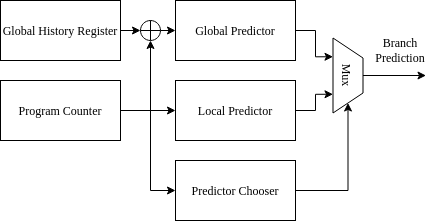
\includegraphics[width=0.45\textwidth]{imgs/overall_design}
    \caption{The overall design of the proposed branch predictor. We have 2 predictors including
    the local and the global predictor for capturing different local/global branch patterns. The
    global predictor is indexed by the xored result between the global history register and the program
    counter. The local predictor is indexed by the program counter only. The predictor chooser select
    the result from both predictor by looking at the current address in the program counter.}
    \label{fig:overall_design}
\end{figure}

\subsection{Local branch predictor}

The presented local branch predictor in our work is based from the implementation in the tournament
predictor. The n least significant bit from program counter is used to index the local history table.
After that, we get the local history from that table. This history is a bit vector of Taken (T/1) and Not-Taken
(N/0), which is used to index the local prediction table. The local prediction table will give the
prediction result based on the state in the table. In this work, we used 2-bit predictors as our
prediction table. This includes 4 possible states including strongly not-taken (SN/00),
weakly not-taken (WN,01), weakly taken (WT/10) and strongly taken (ST/11). The first two states
will give not-taken as the prediction result, while the last two will give taken as the prediction
result. The internal process of this predictor is also shown in Figure \ref{fig:local_predictor}.

\begin{figure}[h]
    \centering
    % \vspace{0.2cm}
    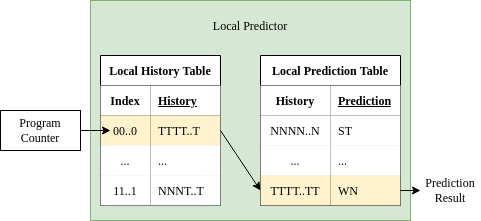
\includegraphics[width=0.48\textwidth]{imgs/local_predictor}
    \caption{The local predictor has two components. First component is the local history table with
    hold the mapping table from address index to local branch history. Then, the obtained branch history
    is used to get the prediction table state which determines the prediction result.}
    \label{fig:local_predictor}
\end{figure}

During the update phase, the history related to the instruction address is updated with the new outcome.
The prediction table state also get updated regarding the new branch outcome. We update the state toward
strongly not-taken and toward strongly taken when the outcome is not-taken and taken respectively. The
update algorithm is shown in Algorithm \ref{alg:local_predictor_update}.

\begin{algorithm}
\caption{An algorithm with caption}\label{alg:local_predictor_update}
\begin{algorithmic}
\Require $n \geq 0$
\Ensure $y = x^n$
\State $y \gets 1$
\State $X \gets x$
\State $N \gets n$
\While{$N \neq 0$}
\If{$N$ is even}
    \State $X \gets X \times X$
    \State $N \gets \frac{N}{2}$  \Comment{This is a comment}
\ElsIf{$N$ is odd}
    \State $y \gets y \times X$
    \State $N \gets N - 1$
\EndIf
\EndWhile
\end{algorithmic}
\end{algorithm}



\subsection{Global branch predictor}

For the global branch predictor, we modified Alpha 21264's global predictor to use the GShare index
instead of just the global history register. The GShare index is calculated by xoring the global history
table with the address in the program counter. This help incorporate both information to select the right
prediction state for the global prediction, i.e., the same address with a different history will point to a
different row in the prediction table. Same as the local branch predictor, the global prediction table stores
2-bit states which related to strongly not-taken, weakly not-taken, weakly taken and strongly taken as described
in the previous section. The internal implementation of this component is shown in Figure \ref{fig:global_predictor}.

\begin{figure}[h]
    \centering
    % \vspace{0.2cm}
    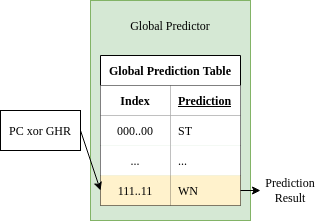
\includegraphics[width=0.3\textwidth]{imgs/global_predictor}
    \caption{The global prediction table is indexed using the xoring result between the program counter and
    the global history register. The prediction result is a 2-bit states which is the same as the prediction
    table used in our local predictor.}
    \label{fig:global_predictor}
\end{figure}

In order to update the global predictor,

\subsection{Predictor chooser}

The predictor chooser is implemented in almost same way as the global branch predictor. The difference is that the chooser
use the instruction address from the program counter as the index, and the 2-bit states determine the
predictor instead. The state 00, 01, 10 and 11 are for strongly local predictor, weakly local predictor,
weakly global predictor and strongly global predictor respectively. The implementation of the predictor chooser
is illustrated in Figure \ref{fig:global_predictor}.

\begin{figure}[h]
    \centering
    % \vspace{0.2cm}
    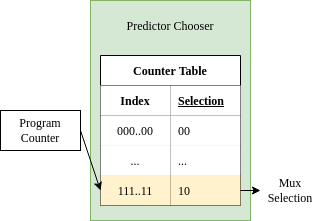
\includegraphics[width=0.3\textwidth]{imgs/predictor_chooser}
    \caption{The global prediction table is indexed using the xoring result between the program counter and
    the global history register. The prediction result is a 2-bit states which is the same as the prediction
    table used in our local predictor.}
    \label{fig:predictor_chooser}
\end{figure}

The chooser's state will be updated if the output from both predictors are different.

\subsection{Predictor Initialization}

\subsection{Storage analysis}

\section{Experimental Setup}

\section{Observation}

\section{Results}

\section{Conclusion}

\subsection{Format Highlights}

Here are the format highlights in a nutshell:
\begin{itemize}
\item Paper must be submitted in printable PDF format.
\item Text must be in a minimum 10pt Times font, see Table~\ref{table:formatting}.
\item Papers must be at most 11 pages (not including references) in a
  two-column format.
\item No page limit for references.
\item Each reference must specify {\em all} authors, i.e., no {\em et al.}
\end{itemize}

\subsection{Paper Evaluation Objectives} 
The committee will make every effort to judge each submitted paper on
its own merits. There will be no target acceptance rate. We expect to
accept a wide range of papers with appropriate expectations for
evaluation --- while papers that build on significant past work with
strong evaluations are valuable, papers that open new areas with less
rigorous evaluation are equally welcome and especially encouraged. We
also acknowledge the wide range of evaluation methodologies in ISCA including
modeling, simulation, prototyping, experimental implementation, real
product evaluation, etc. 

\section{Paper Preparation Instructions}

\subsection{Paper Formatting}
Papers must be submitted in printable PDF format and should contain a
{\em maximum of 11 pages} of single-spaced two-column text, {\bf not
  including references}.  You may include any number of pages for
references, but see below for more instructions.  If you are using
\LaTeX~\cite{lamport94} to typeset your paper, then we suggest that
you use the template used to prepare this document, which you can find
on the ISCA 2020 website. If you use a different
software package to typeset your paper, then please adhere to the
guidelines given in Table~\ref{table:formatting}.  

\begin{scriptsize}
\begin{table}[h!]
  \centering
  \caption{Formatting guidelines for submission.}
  \label{table:formatting}
  \begin{tabular}{|l|l|}
    \hline
    \textbf{Field} & \textbf{Value}\\
    \hline
    \hline
    File format & PDF \\
    \hline
    Page limit & 11 pages, {\bf not including}\\
               & {\bf references}\\
    \hline
    Paper size & US Letter 8.5in $\times$ 11in\\
    \hline
    Top margin & 1in\\
    \hline
    Bottom margin & 1in\\
    \hline
    Left margin & 0.75in\\
    \hline
    Right margin & 0.75in\\
    \hline
    Body & 2-column, single-spaced\\
    \hline
    Space between columns & 0.25in\\
    \hline
    Line spacing (leading) & 11pt \\
    \hline
    Body font & 10pt, Times\\
    \hline
    Abstract font & 10pt, Times\\
    \hline
    Section heading font & 12pt, bold\\
    \hline
    Subsection heading font & 10pt, bold\\
    \hline
    Caption font & 9pt (minimum), bold\\
    \hline
    References & 8pt, no page limit, list \\
               & all authors' names\\
    \hline
  \end{tabular}
\end{table}
\end{scriptsize}

{\em Please ensure that you include page numbers with your
  submission}. This makes it easier for the reviewers to refer to
different parts of your paper when they provide comments. Please
ensure that your submission has a banner at the top of the title page,
similar to this document, which contains the submission number and the
notice of confidentiality.  If using the template, just replace `NaN'
with your submission number. 

\subsection{Content}
Reviewing will be {\em double blind} (no author list); therefore,
please do not include any author names on any submitted documents
except in the space provided on the submission form.  You must also
ensure that the metadata included in the PDF does not give away the
authors. If you are improving upon your prior work, refer to your
prior work in the third person and include a full citation for the
work in the bibliography.  For example, if you are building on {\em
  your own} prior work in the
papers~\cite{nicepaper1,nicepaper2,nicepaper3}, you would say
something like: "While the authors of~\cite{nicepaper1,nicepaper2,nicepaper3} did X,
Y, and Z, this paper additionally does W, and is therefore much
better."  Do NOT omit or anonymize references for blind review.  There
is one exception to this for your own prior work that appeared in IEEE
CAL, arXiv, workshops without archived proceedings, etc.\ as
discussed later in this document. 

\noindent\textbf{Figures and Tables:} Ensure that the figures and
tables are legible.  Please also ensure that you refer to your figures
in the main text.  Many reviewers print the papers in
gray-scale. Therefore, if you use colors for your figures, ensure that
the different colors are highly distinguishable in gray-scale. 

\noindent\textbf{References:}  There is no length limit for
references. {\em Each reference must explicitly list all authors of
  the paper.  Papers not meeting this requirement will be rejected.}
Since there is no length limit for the number of pages
used for references, there is no need to save space here. 


\section{Paper Submission Instructions}

\subsection{Guidelines for Determining Authorship}
IEEE guidelines dictate that authorship should be based on a {\em
  substantial intellectual contribution}. It is assumed that all
authors have had a significant role in the creation of an article that
bears their names. In particular, the authorship credit must be
reserved only for individuals who have met each of the following
conditions: 

\begin{enumerate}
\item Made a significant intellectual contribution to the theoretical
  development, system or experimental design, prototype development,
  and/or the analysis and interpretation of data associated with the
  work contained in the article; 

\item Contributed to drafting the article or reviewing and/or revising
  it for intellectual content; and 

\item Approved the final version of the article as accepted for publication, including references.
\end{enumerate}

A detailed description of the IEEE authorship guidelines and
responsibilities is available online.\footnote{\url{https://www.ieee.org/publications_standards/publications/rights/Section821.html}} Per
these guidelines, it is not acceptable to award {\em honorary}
authorship or {\em gift} authorship. Please keep these guidelines in
mind while determining the author list of your paper. 

\subsection{Declaring Authors}
Declare all the authors of the paper upfront. Addition/removal of
authors once the paper is accepted will have to be approved by the
program chair, since it potentially undermines the goal of eliminating
conflicts for reviewer assignment. 

\subsection{Areas and Topics}
Authors should indicate specific topics covered by the paper on the
submission page. If you are unsure whether your paper falls within the
scope of ISCA, please check with the program chair --- ISCA is a broad,
multidisciplinary conference and encourages new topics. 

\subsection{Declaring Conflicts of Interest}

Authors must register all their conflicts on the paper submission
site. Conflicts are needed to ensure appropriate assignment of
reviewers. If a paper is found to have an undeclared conflict that
causes a problem OR if a paper is found to declare false conflicts in
order to abuse or `game' the review system, the paper may be rejected. 

Please declare a conflict of interest with the following people for any author of your paper.
A conflict occurs in the following cases:
\begin{enumerate}
\item Between advisor and advisee forever. 
\item Between family members forever. 
\item Between people who have collaborated in the last 5 years. This
  collaboration can consist of a joint research or development
  project, a joint paper, or when there is direct funding from the
  potential reviewer (as opposed to company funding) to an author of
  the paper. Co-participation in professional activities, such as
  tutorials or studies, is not cause for conflict. When in doubt, the
  author should check with the Program Chair. 
\item Between people from same institution or who were in the same
  institution in the last 5 years.  
\item Between people whose relationship prevents the reviewer from
  being objective in his/her assessment. 
\end{enumerate}

`Service' collaborations, such as co-authoring a report for a
professional organization, serving on a program committee, or
co-presenting tutorials, do not themselves create a conflict of
interest. Co-authoring a paper that is a compendium of various
projects with no true collaboration among the projects does not
constitute a conflict among the authors of the different projects. On
the other hand, there may be others not covered by the above with whom
you believe a COI exists, for example, an ongoing collaboration which
has not yet resulted in the creation of a paper or proposal. Please
report such COIs; however, you may be asked to justify them. Please be
reasonable. For example, you cannot declare a COI with a reviewer just
because that reviewer works on topics similar to or related to those
in your paper.  The program chair may contact co-authors to explain a COI
whose origin is unclear. 

Most reviews will be solicited among the members of the PC and the ERC, but other
members from the community may also write reviews. Please declare all
your conflicts (not just restricted to the PC and ERC) on the
submission form. When in doubt, contact the program chair. 


\subsection{Concurrent Submissions and Workshops}
By submitting a manuscript to ISCA 2020, the authors guarantee that
the manuscript has not been previously published or accepted for
publication in a substantially similar form in any conference,
journal, or the archived proceedings of a workshop (e.g., in the
ACM/IEEE digital libraries) --- see exceptions below. The authors also
guarantee that no paper that contains significant overlap with the
contributions of the submitted paper will be under review for any
other conference or journal or an archived proceedings of a workshop
during the ISCA 2020 review period. Violation of any of these
conditions will lead to rejection. 

The only exceptions to the above rules are for the authors' own papers
in (1) workshops without archived proceedings such as in the ACM/IEEE
digital libraries (or where the authors chose not to have their paper
appear in the archived proceedings), or (2) venues such as IEEE CAL or
arXiv where there is an explicit policy that such publication does not
preclude longer conference submissions.  In all such cases, the
submitted manuscript may ignore the above work to preserve author
anonymity. This information must, however, be provided on the
submission form --- the program chair will make this information available
to reviewers if it becomes necessary to ensure a fair review.  As
always, if you are in doubt, it is best to contact program chairs. 


Finally, the ACM/IEEE Plagiarism Policies\footnote{\url{http://www.acm.org/publications/policies/plagiarism_policy}\\
\url{https://www.ieee.org/publications_standards/publications/rights/plagiarism_FAQ.html}}
cover a range of ethical issues concerning the misrepresentation of
other works or one's own work. 


\section*{Acknowledgements}
This document is derived from previous conferences, in particular ISCA
2019 and MICRO 2019.

%%%%%%% -- PAPER CONTENT ENDS -- %%%%%%%%


%%%%%%%%% -- BIB STYLE AND FILE -- %%%%%%%%
\bibliographystyle{IEEEtranS}
\bibliography{refs}
%%%%%%%%%%%%%%%%%%%%%%%%%%%%%%%%%%%%

\end{document}

